\documentclass[a4paper,dvipsnames]{article}

\input ../header
\newcommand{\checkedbox}{\makebox[0pt][l]{$\square$}\raisebox{.15ex}{\hspace{0.1em}$\checkmark$}}
\newcommand{\checkbox}{\makebox[0pt][l]{$\square$}\raisebox{.15ex}{\hspace{0.1em}}\hspace{3mm}}

\begin{document}

\title{Évaluation 4 -- Sujet A}
\author{}
\date{}

\maketitle{}

\pagestyle{empty}

\exo\vspace{-2mm} 
\begin{enumerate}
  \item Écrire chaque nombre sous la forme $a\sqrt{b}$, où $a$ est un entier et $b$ l'entier naturel le plus petit possible.

    \begin{multicols}{3}
      \begin{enumerate}
	\item $\sqrt{75}$
	\item $\sqrt{15}\times\sqrt{20}$
	\item $3\sqrt{3}-2\sqrt{12}+\sqrt{300}$
      \end{enumerate}
    \end{multicols}
  \item Écrire sans racine carrée au dénominateur :

    \begin{multicols}{2}
      \begin{enumerate}
	\item $\dfrac{3}{\sqrt{7}}$
	\item $\dfrac{5}{\sqrt{6}-1}$
      \end{enumerate} 
    \end{multicols}

  \item Donner une valeur arrondie de $\dfrac{3}{\sqrt{7}}$ à $10^{-3}$ près, puis un encadrement d'amplitude $10^{-4}$ de $\dfrac{5}{\sqrt{6}-1}$.
\end{enumerate}

\bigskip

\exo On fait tourner chacune des roulettes suivantes et on note la couleur obtenue. Modéliser chaque expérience aléatoire en complétant le tableau donné.

\begin{multicols}{2}
  \begin{center}
    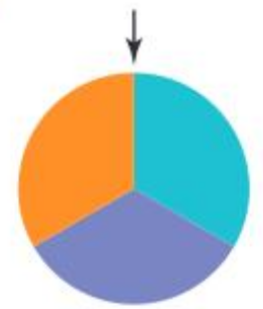
\includegraphics[width=2.5cm]{evaluation_4_figure_1.png}
  \end{center}

  \begin{center}
    \vspace*{0.7cm}
    \hspace*{-3cm}\begin{tabular}{@{}cccc@{}}
      \toprule
      Couleur obtenue & vert & orange & bleu\\
      \midrule
      Probabilité & & & \vphantom{$\dfrac{1}{4}$}\\
      \bottomrule
    \end{tabular}
  \end{center}
\end{multicols}

\begin{multicols}{2}
  \begin{center}
    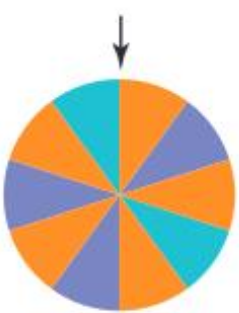
\includegraphics[width=2.3cm]{evaluation_4_figure_3.png}
  \end{center}

  \begin{center}
    \vspace*{0.75cm}
    \hspace*{-3cm}\begin{tabular}{@{}cccc@{}}
      \toprule
      Couleur obtenue & vert & orange & bleu\\
      \midrule
      Probabilité & & & \vphantom{$\dfrac{1}{4}$}\\
      \bottomrule
    \end{tabular}
  \end{center}
\end{multicols}

\bigskip

\exo On considère la fonction (incomplète) suivante écrite en Python :

\begin{minted}{python}
def mystere(B, b, h):
    a = ...
    return ...
\end{minted}

\begin{enumerate}
  \item Comment s'appelle cette fonction ?
  \item Combien de paramètres possède-t-elle ?
  \item Quel mot-clé permet de définir une fonction en Python ?
  \item Compléter la fonction afin qu'elle renvoie l'aire d'un trapèze de bases $B$ et $b$, et de hauteur $h$.\\
    \textit{Remarque. -- On rappelle que l'aire d'un tel trapèze est donnée par la formule :
      \[\dfrac{(B + b)\times h}{2}.\]
  }
\item Comment utiliser cette fonction pour calculer l'aire d'un trapèze de bases $7$ et $5$, et de hauteur $3$ ?
\end{enumerate}

\end{document}
